\chapter{控制器仿真实验结果分析}%TODO:仿真需要给出控制器的相关参数,以及初始条件等等。
\label{chap:simulatin_expermient}
上一章介绍了无人机编队控制器的仿真环境,
则本章中,按照第\ref{chap:controller_design}
章中给出的控制器的数学模型,选定相应的初始条件进行双机的质点模型数学仿真:即不考虑无人机的姿态,只考虑无人机的位置,速度大小以及方向。
之后,利用第\ref{chap:hardware}章中介绍的$ROS/Gazebo-PX4$仿真环境,在考虑无人机动力学的条件下进行双机编队仿真。
\section{基于MATLAB/Simulink的双机编队数学仿真}
本节数学仿真只验证编队控制器的控制性能以及控制逻辑的正确性,因而在仿真之前,做如下假设:
\begin{enumerate}
\item 无人机自动驾驶仪内环仅为一个具有时间常数$\tau$一阶惯性环节。
\item 无人机的姿态动力学没有过渡过程,即姿态动力学方程由相应的稳态方程代替。
\end{enumerate}
另外,按照第\ref{chap:controller_design}章中控制器设计分为水平平面以及竖直平面的原则,本节之中的仿真也是分为两个方面进行的;在任何
在其中任意一个平面内仿真时,都假设另外一个平面已经达到了控制目标,并且处于稳态。

在水平面的仿真中:选取的初始条件均为在地面坐标系NED中定义,其值如下表所示:
\begin{table}[H]
    \centering
    \caption{水平面内数学仿真初始运动学量} \label{tab:matlab_init_cond}
    \begin{tabular*}{0.9\textwidth}{@{\extracolsep{\fill}}c|cccc}
        \toprule
        指标     & 初速度(m/s)   & 初始位置(m)    & 航迹角(°) & 高度(m)  \\
        \midrule
        领机     & (20.0,0.0)  & (-50.0,100.0) & 0.0        & 100.0 \\
        从机     & (10.0,10.0) & (0.0,100.0)  & 45.0       & 0.0   \\
        \bottomrule
    \end{tabular*}
\end{table}
水平面内的编队控制器的参数,包括两个通道的误差混合参数以及增量式PID的参数:
\begin{table}[H]
    \centering
    \caption{水平面内编队控制器参数} \label{tab:matlab_PID_param}
    \begin{tabular*}{0.9\textwidth}{@{\extracolsep{\fill}}c|ccccc}
        \toprule
        参数 & 比例$K_P$     & 积分$K_I$    & 微分$K_D$ & 混合参数1 & 混合参数2  \\
        \midrule
        X & 0.5 & 0.01  & 0.008  & 0.45  & 0.65 \\
        Y & 0.7 & 0.005 & 0.0015 & 0.008 & 0.5 \\
        \bottomrule
    \end{tabular*}
\end{table}

仿真的结果如下三图所示:其中,图\ref{fig:c5-matlab-pos},表示双机编队位置关系,横轴为NED坐标系下的E轴,纵轴为N轴。
图\ref{fig:c5-matlab-vel}以及图\ref{fig:c5-matlab-eta}分别表示双机速度大小以及速度方向的与时间的关系图。由仿真结果可得,
在算法层面上,第\ref{chap:controller_design}所设计的编队控制器在水平平面内可以完成编队控制的任务。
\begin{figure}[H]
    \centering
    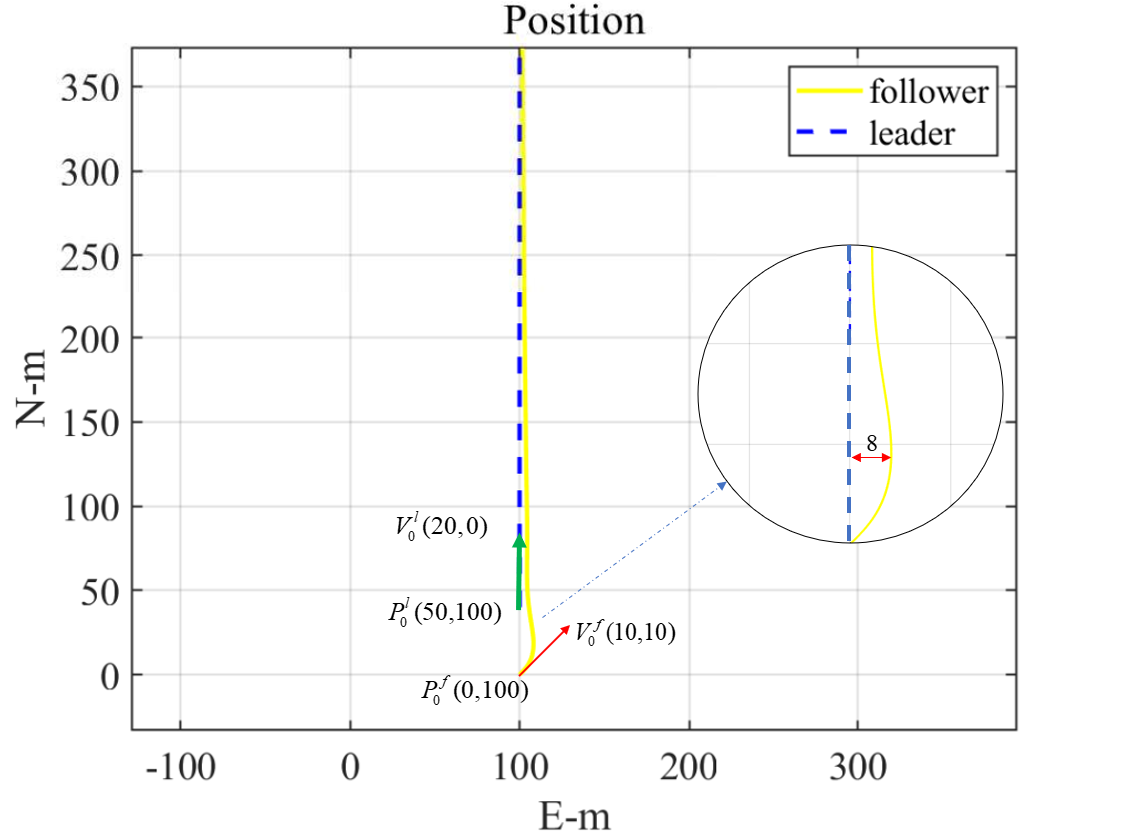
\includegraphics[width=0.85\textwidth]{figures/c5/c5-matlab-pos.png}
    \caption{水平面双机编队位置关系}\label{fig:c5-matlab-pos}
\end{figure}
\begin{figure}[H]
    \centering
    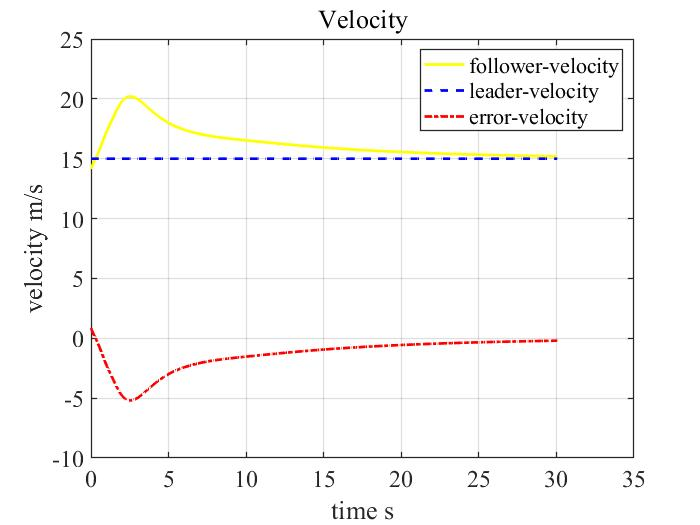
\includegraphics[width=0.85\textwidth]{figures/c5/c5-matlab-vel.jpg}
    \caption{水平面双机速度大小关系}\label{fig:c5-matlab-vel}
\end{figure}
\begin{figure}[H]
    \centering
    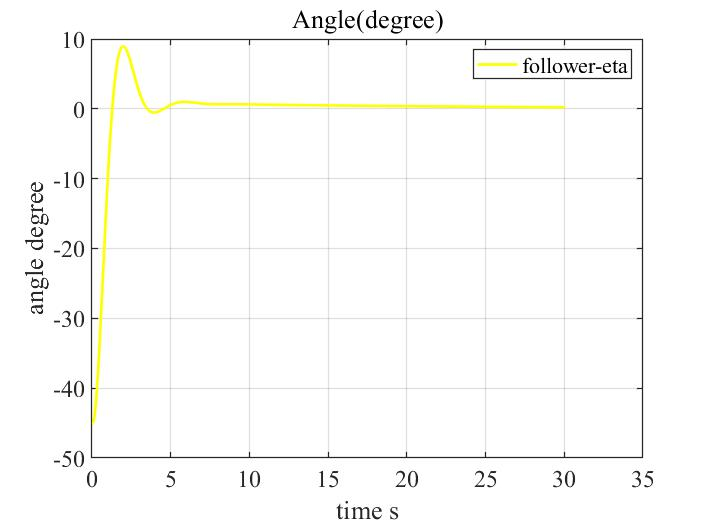
\includegraphics[width=0.85\textwidth]{figures/c5/c5-matlab-eta}
    \caption{水平面双机航迹角关系}\label{fig:c5-matlab-eta}
\end{figure}

竖直平面内,由于控制器的任务是消除高度误差以及追踪来自水平平面控制器的期望速度,控制量将是期望推力$T^{des}$以及期望俯仰角$\theta^{des}$,因而需要引入竖直平面内的无人机动力学模型(参见式\ref{point_dynamaic});按照之前的假设,无人机姿态内环为理想环节,可以用一个时间常数为$\tau_{\theta}$的惯性环节代替之。再结合式\ref{fol_motion_eauation},可以进行竖直平面的相关仿真:
仿真时的领机从机初始运动学量为:
\begin{table}[H]
    \centering
    \caption{竖直面内数学仿真初始运动学量} \label{tab:matlab_vel_cond}
    \begin{tabular*}{0.9\textwidth}{@{\extracolsep{\fill}}c|cc}
        \toprule
        指标 & 初速度(m/s)    & 初始高度(m)\\
        \midrule
        领机 & 20.0  & 10.0\\
        从机 & 10.0 & 100.0\\
        \bottomrule
    \end{tabular*}
\end{table}
竖直内TECS控制器的参数如下表所示:
\begin{table}[H]
    \centering
    \caption{竖直面内TECS控制器参数} \label{tab:matlab_TECS_param}
    \begin{tabular*}{0.9\textwidth}{@{\extracolsep{\fill}}c|cccc}
        \toprule
        TECS参数 & 油门时间常数 & 俯仰角时间常数 & 俯仰角阻尼 & 油门阻尼   \\
        \midrule
        值       & 4.0            & 3.0              & 0.7        & 0.65   \\
        \bottomrule
    \end{tabular*}
\end{table}
\begin{table}[H]
    \centering
    \caption{竖直面内TECS控制器参数(续表)} \label{tab:matlab_TECS_param_app}
    \begin{tabular*}{1.0\textwidth}{@{\extracolsep{\fill}}c|cccc}
        \toprule
        TECS参数 & 积分增益 & 俯仰角-速度比重常数 & 高度误差比例增益 & 速度误差比例增益  \\
        \midrule
        值       & 0.3      & 1.0                   & 0.05             & 0.02     \\
        \bottomrule
    \end{tabular*}
\end{table}

为了方便读图,现在将$NED$坐标系下的$D$轴取反之后并用“$height$”表示,
仿真的结果如下三图所示:
\begin{figure}[H]
    \centering
    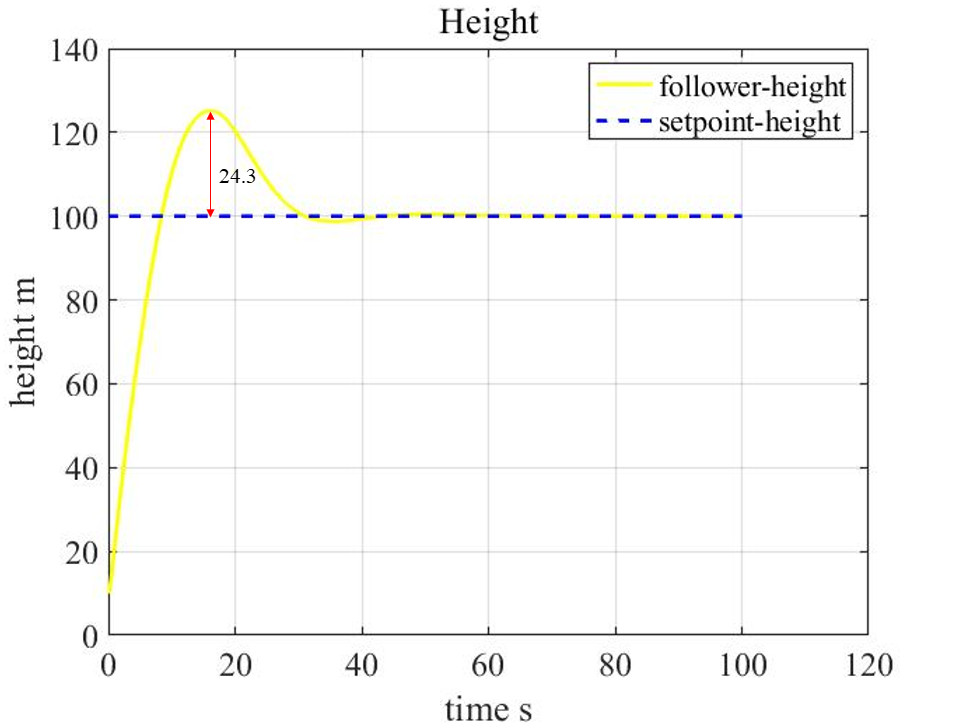
\includegraphics[width=0.85\textwidth]{figures/c5/c5-TECS-height.jpg}
    \caption{竖直平面高度关系}\label{fig:c5-TECS-height}
\end{figure}
\begin{figure}[H]
    \centering
    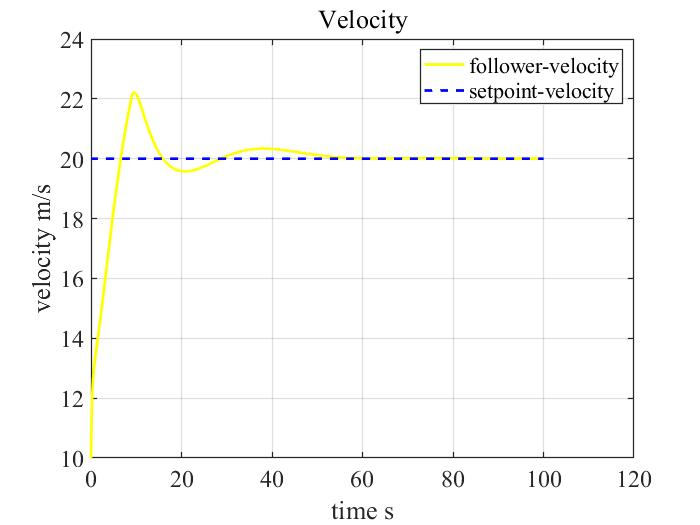
\includegraphics[width=0.85\textwidth]{figures/c5/c5-TECS-vel.jpg}
    \caption{竖直平面速度关系}\label{fig:c5-TECS-vel}
\end{figure}
\begin{figure}[H]
    \centering
    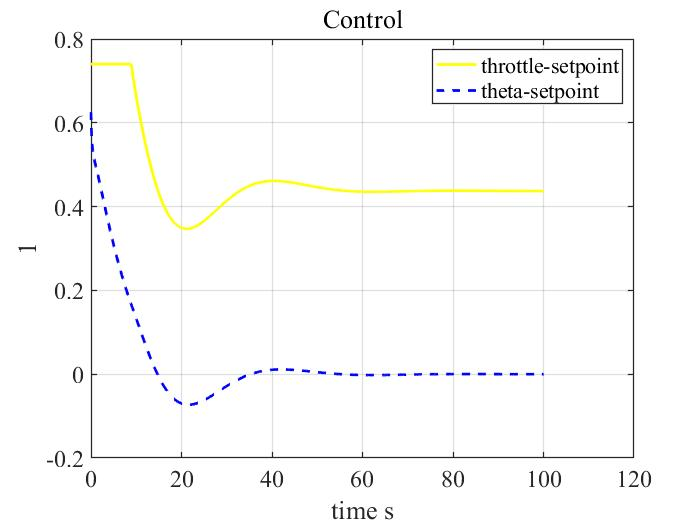
\includegraphics[width=0.85\textwidth]{figures/c5/c5-TECS-control.jpg}
    \caption{竖直平面控制量关系}\label{fig:c5-TECS-control}
\end{figure}
由仿真结果可知,本文所设计的TECS控制器可以完成对于期望速度以及期望高度的跟踪,从而达到消除竖直平面内的误差的作用。
\section{基于ROS/Gazebo-PX4的双机编队动力学仿真}
根据第\ref{chap:hardware}章中介绍的ROS-Gazebo仿真环境,进行仿真环境下的双机编队飞行试验。首先利用QGround Control 地面站为领机规划
一条包括起飞以及降落航点在内的一条长直航线。之后先使用地面站将领机1(vehicle 1)
解锁,切换任务模式之后起飞,按照既定航线飞行。等待领机到达第一个
航点之后,再起飞从机2(vehicle 2)
,并切换到外部控制模式,即编队控制的控制逻辑。之后经过一段时间的飞行之后,采集飞行之中的编队误差等数据:最终
编队稳定之后的可视化效果如下:
\begin{figure}[H]
    \centering
    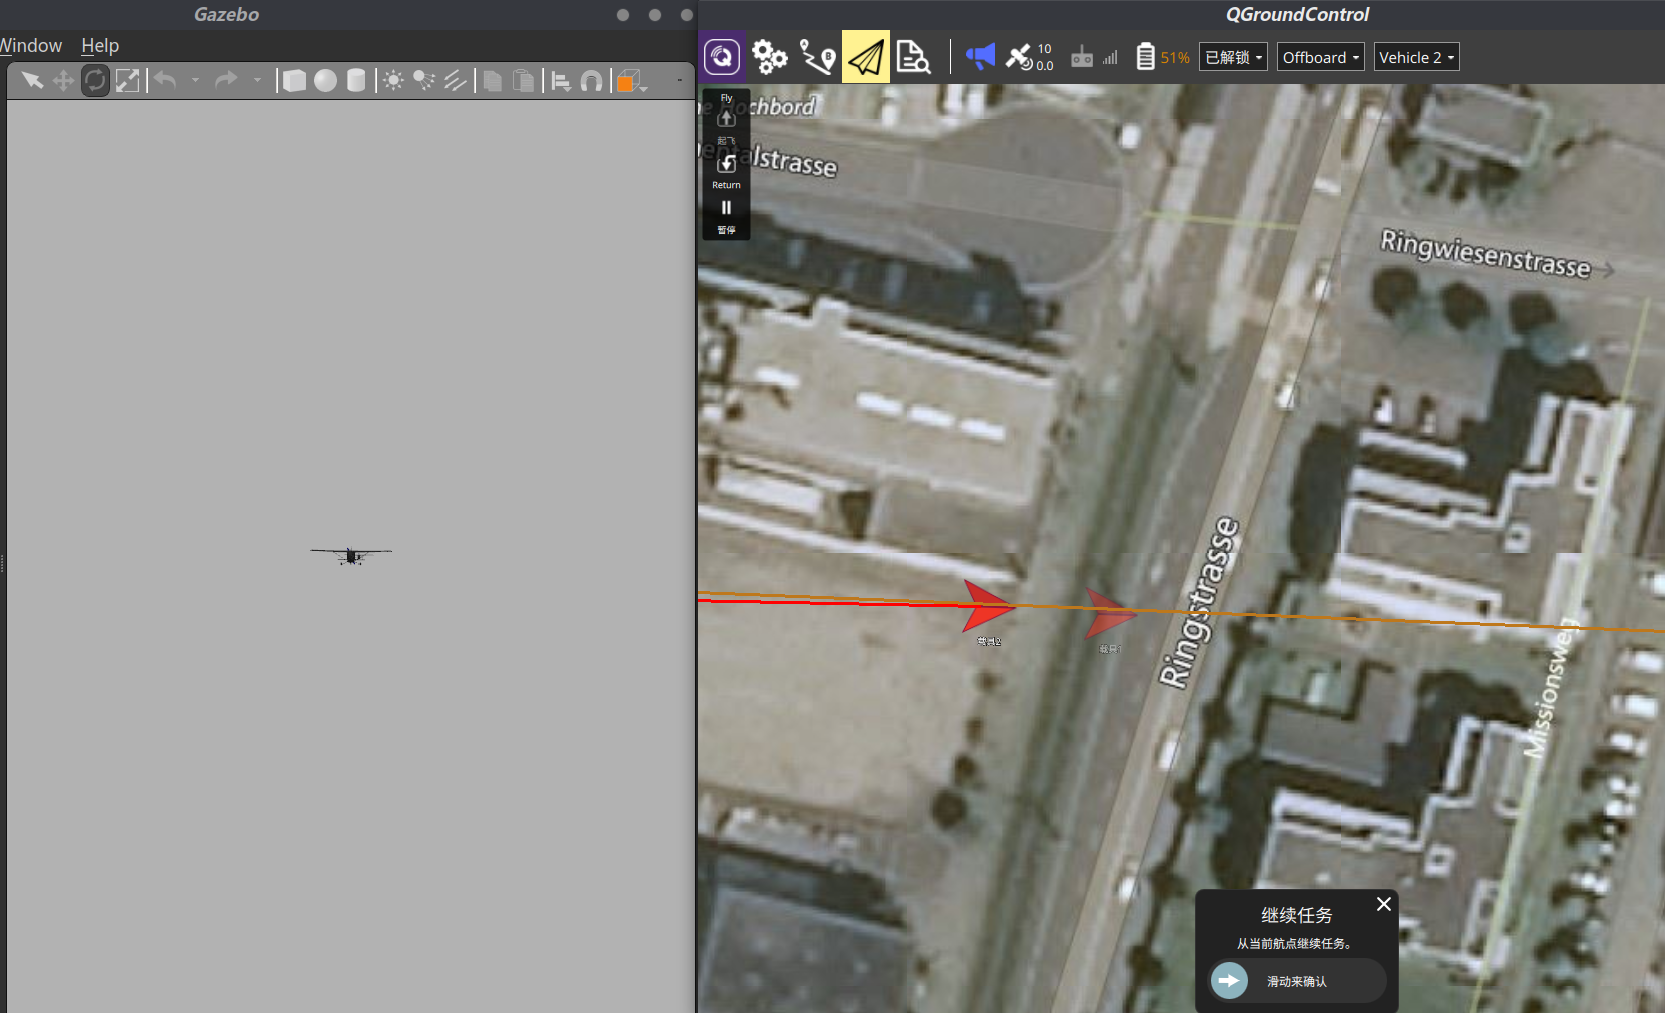
\includegraphics[width=0.85\textwidth]{figures/c5/c5-real-overview}
    \caption{稳定编队之后的编队可视化效果}\label{c5-real-overview}
\end{figure}
动力学仿真的初始条件如下表所示:
\begin{table}[H]
    \centering
    \caption{Gazebo双机编队动力学仿真初始条件} \label{tab:real_init_cond}
    \begin{tabular*}{0.9\textwidth}{@{\extracolsep{\fill}}c|cccc}
        \toprule
        指标     & 初速度(m)     & 初始位置(m)  & 航迹角(°) & 高度(m)  \\
        \midrule
        领机     & (0.0,0.0)    & (0.0,80.0) & 90    & 100.0 \\
        从机     & (0.0,15.0) & (0.0,0.0)   & 90    & 0.0   \\
        \bottomrule
    \end{tabular*}
\end{table}
仿真过程中的编队控制器的控制器参数如下表所示:
\begin{table}[H]
    \centering
    \caption{水平面内控制器参数} \label{tab:matlab_PID_param}
    \begin{tabular*}{0.9\textwidth}{@{\extracolsep{\fill}}c|ccccc}
        \toprule
        参数 & 比例$K_P$     & 积分$K_I$    & 微分$K_D$ & 混合参数1 & 混合参数2  \\
        \midrule
        X & 0.3 & 0.01  & 0.008  & 0.4   & 0.65 \\
        Y & 0.4 & 0.005 & 0.0015 & 0.005 & 0.4 \\
        \bottomrule
    \end{tabular*}
\end{table}
TECS控制器的参数如下表所示:
\begin{table}[H]
    \centering
    \caption{竖直面内TECS控制器参数} \label{tab:matlab_TECS_param}
    \begin{tabular*}{0.9\textwidth}{@{\extracolsep{\fill}}c|cccc}
        \toprule
        TECS参数 & 油门时间常数 & 俯仰角时间常数 & 俯仰角阻尼 & 油门阻尼   \\
        \midrule
        值       & 8            & 5              & 0.3        & 0.5   \\
        \bottomrule
    \end{tabular*}
\end{table}
\begin{table}[H]
    \centering
    \caption{竖直面内TECS控制器参数(续表)} \label{tab:matlab_TECS_param_app}
    \begin{tabular*}{1.0\textwidth}{@{\extracolsep{\fill}}c|cccc}
        \toprule
        TECS参数 & 积分增益 & 俯仰角-速度比重常数 & 高度误差比例增益 & 速度误差比例增益  \\
        \midrule
        值      & 0.1  & 1          & 0.05     & 0.02     \\
        \bottomrule
    \end{tabular*}
\end{table}
在仿真过程中,利用ROS提供的rosbag等数据记录工具,可以进行仿真之中的数据记录与处理:
图\ref{c5-real-pos_err_x}-图\ref{c5-real-pos_err_z}分别代表了双机编队位置误差投影
在从机坐标系$O_kx_ky_kz_k$中的分量随时间的变化关系;图\ref{c5-real-eta_err}代表从
机与领机的速度方向误差随时间变化关系;图\ref{c5-real-vel_err}代表从机与领机的速度大小误差随时间的变化关系。
\begin{figure}[H]
    \centering
    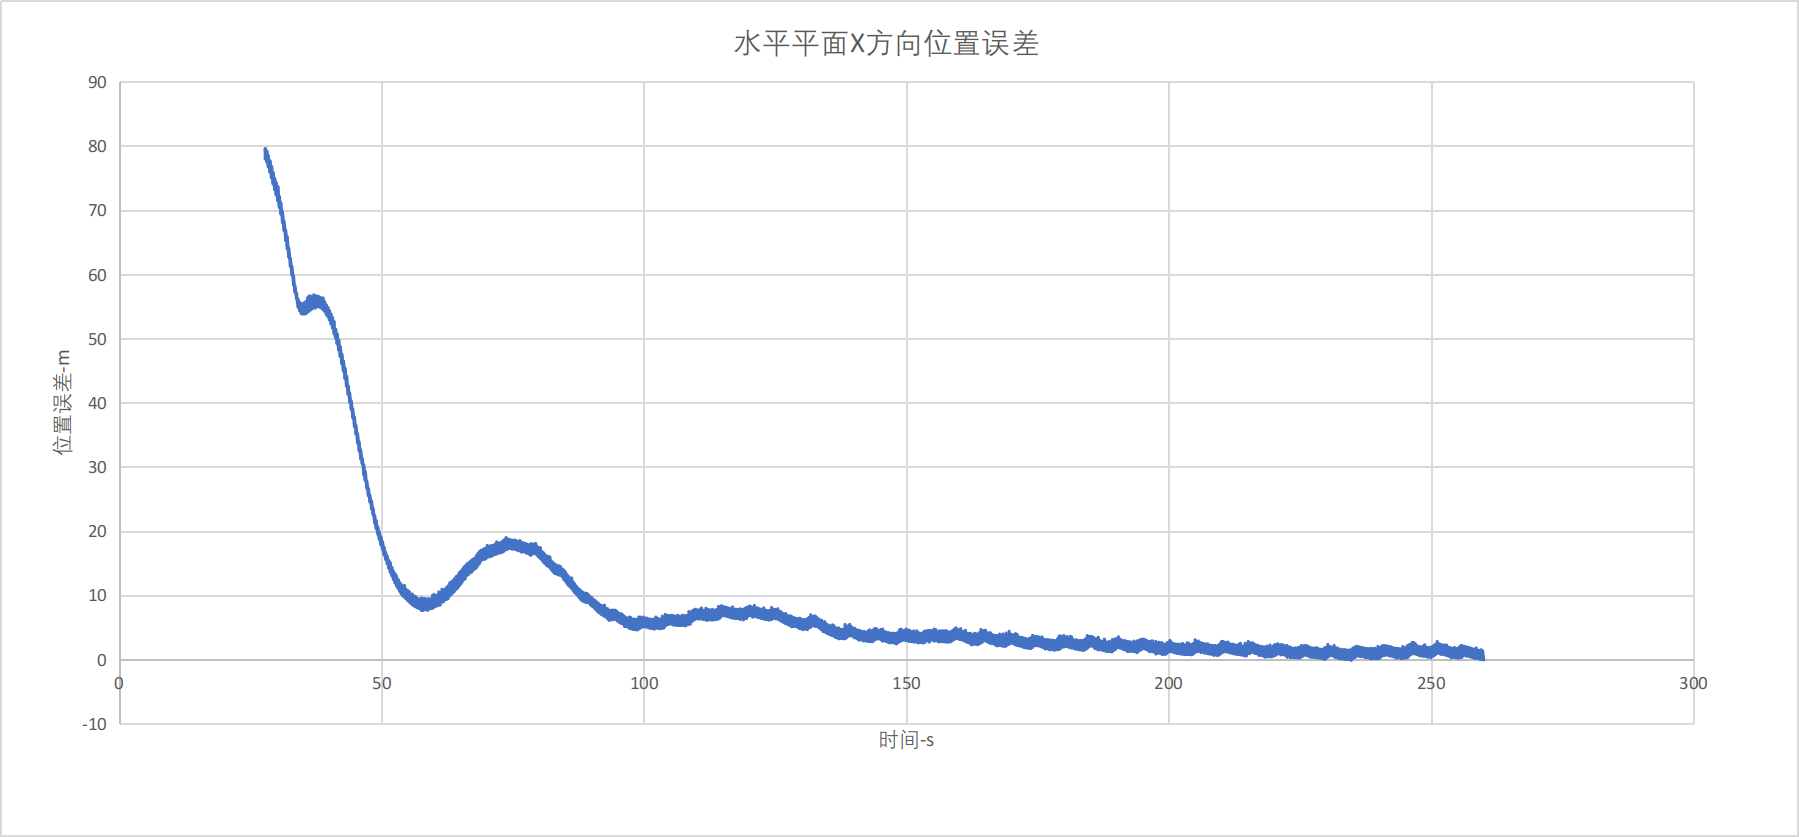
\includegraphics[width=0.85\textwidth]{figures/c5/c5-real-pos_err_x}
    \caption{X通道位置误差}\label{c5-real-pos_err_x}
\end{figure}
\begin{figure}[H]
    \centering
    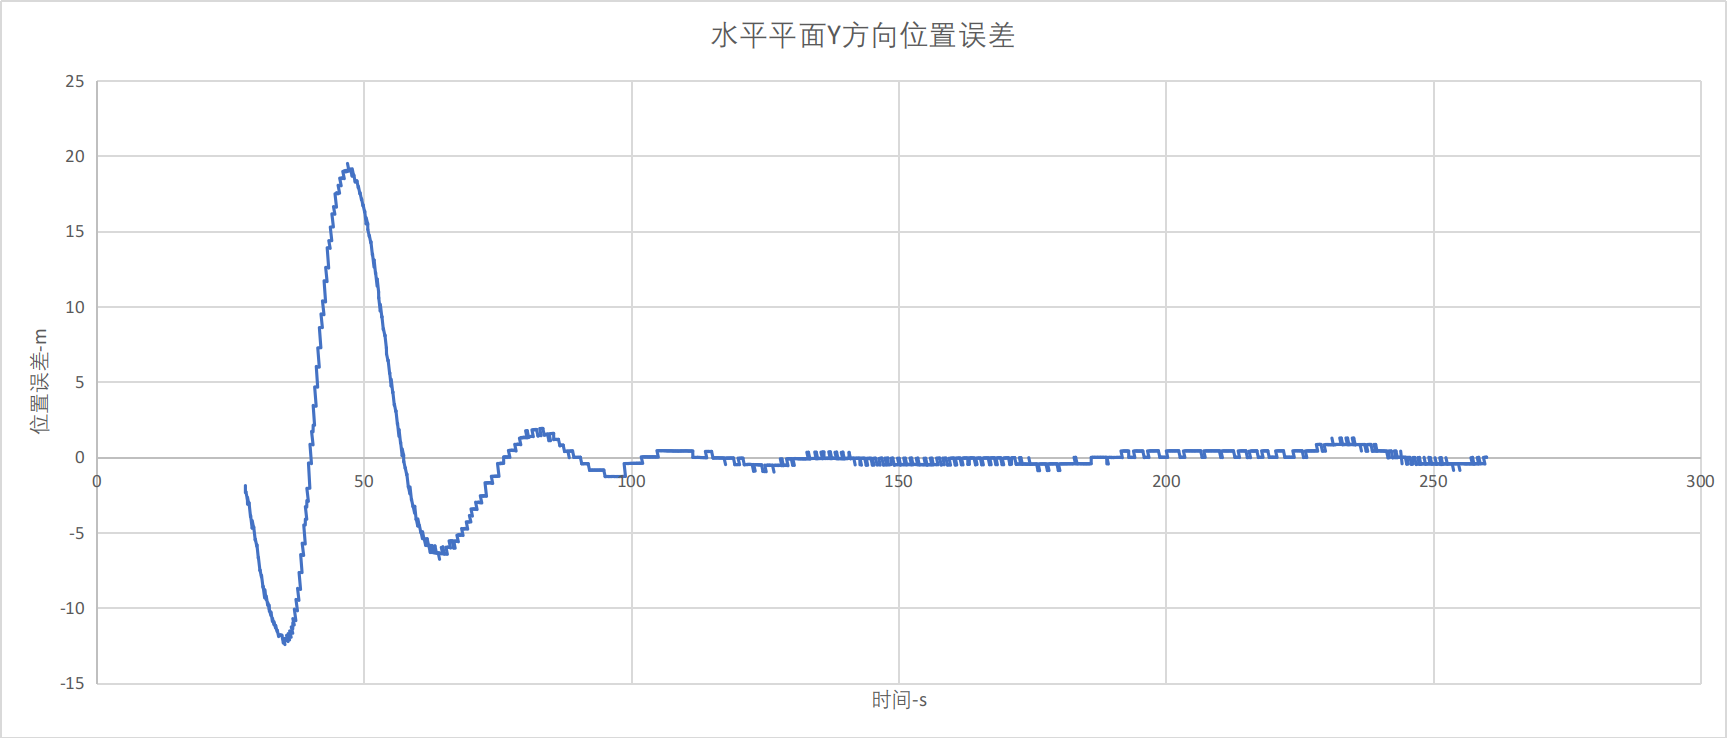
\includegraphics[width=0.85\textwidth]{figures/c5/c5-real-pos_err_y}
    \caption{Y通道位置误差}\label{c5-real-pos_err_y}
\end{figure}
\begin{figure}[H]
    \centering
    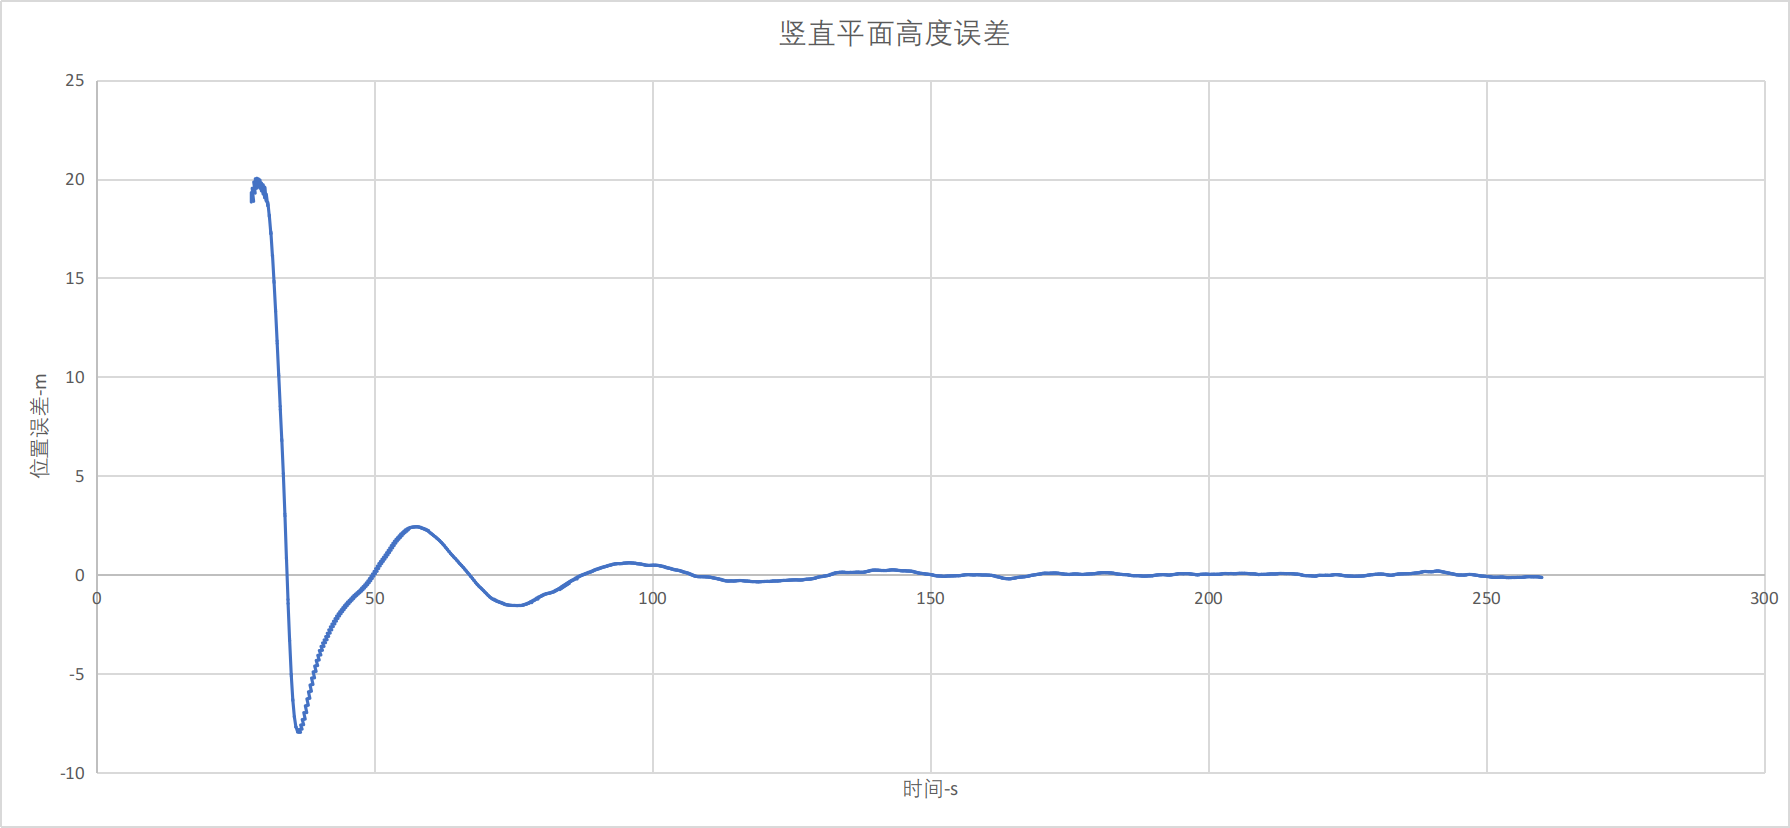
\includegraphics[width=0.85\textwidth]{figures/c5/c5-real-pos_err_z}
    \caption{Z通道位置误差}\label{c5-real-pos_err_z}
\end{figure}
\begin{figure}[H]
    \centering
    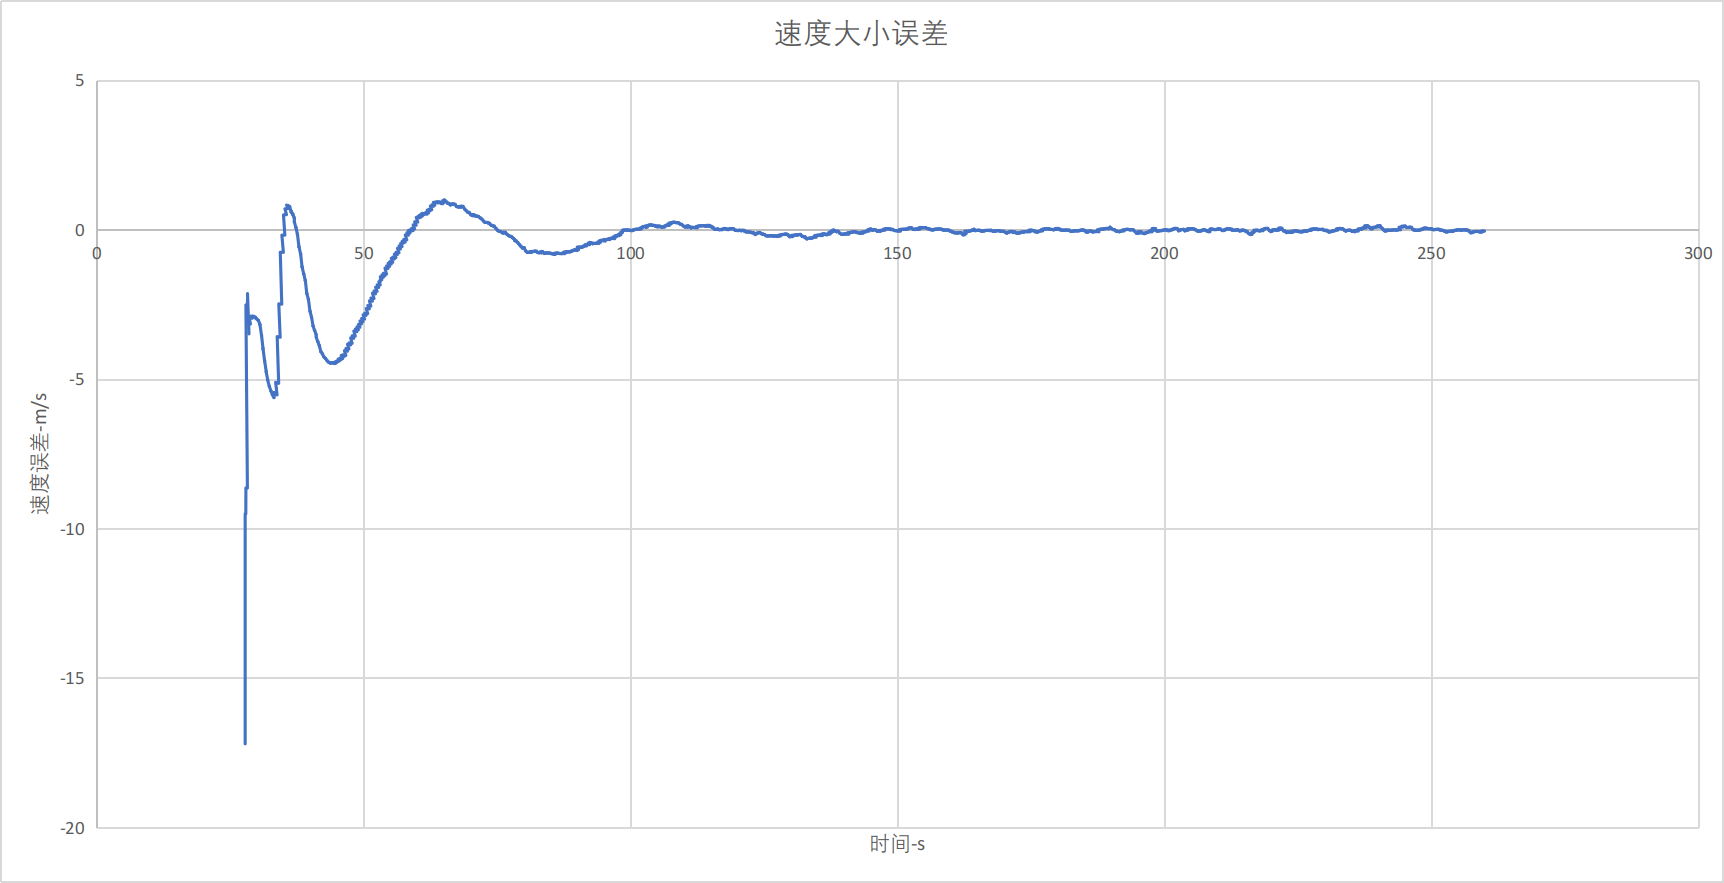
\includegraphics[width=0.85\textwidth]{figures/c5/c5-real-vel_err}
    \caption{领机从机速度大小误差}\label{c5-real-vel_err}
\end{figure}
\begin{figure}[H]
    \centering
    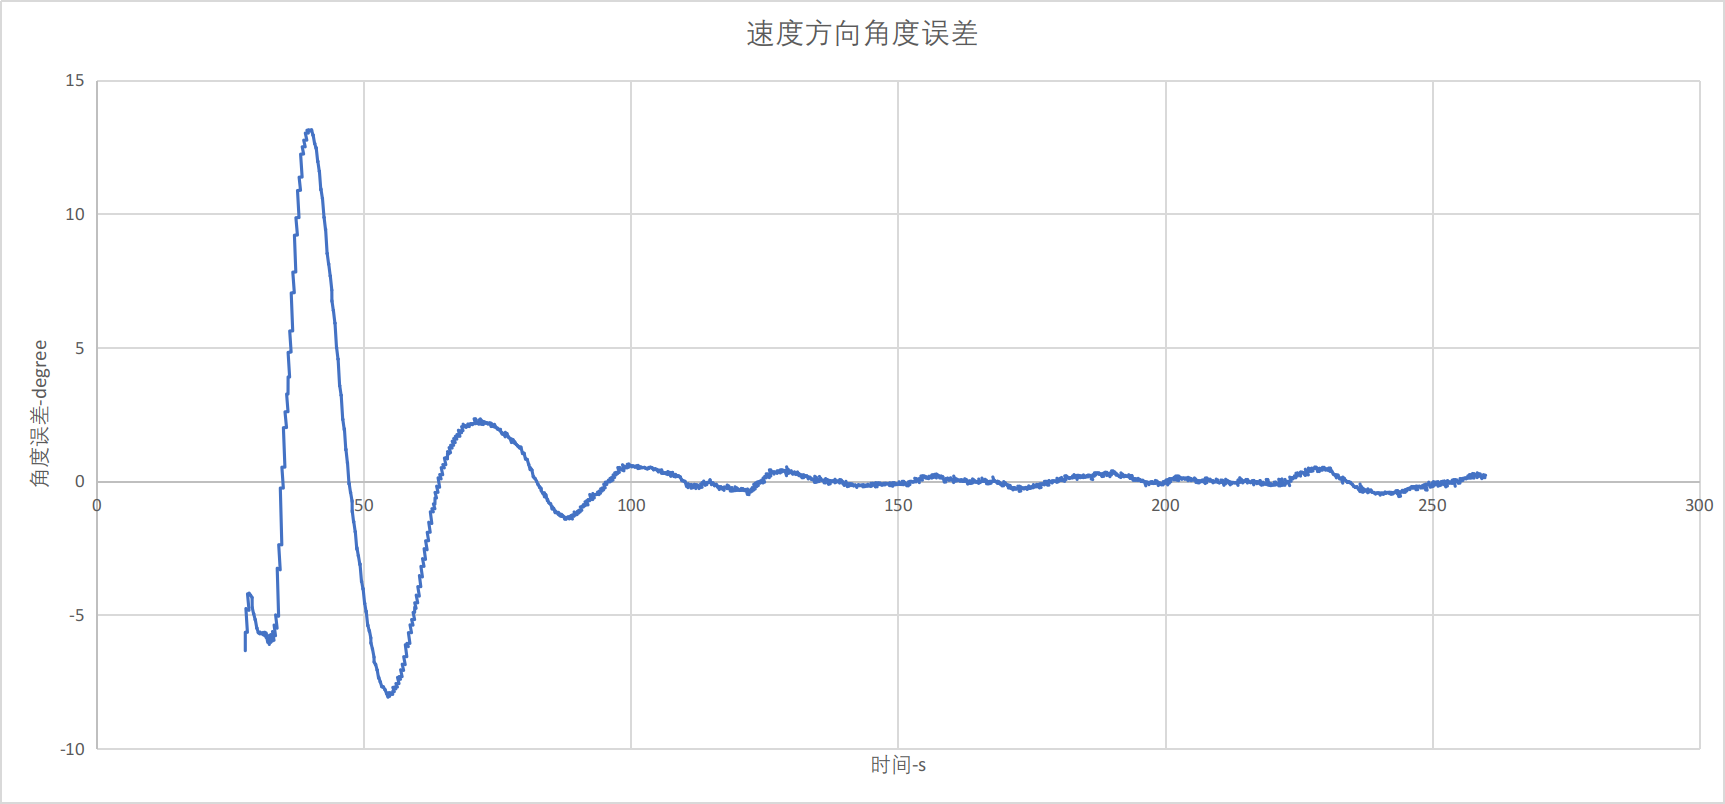
\includegraphics[width=0.85\textwidth]{figures/c5/c5-real-eta_err}
    \caption{领机从机航迹角误差}\label{c5-real-eta_err}
\end{figure}
需要注意的一点是:此处的位置误差指的是从机的实际位置与编队的期望位置之间的位值误差,而并非与领机的位置误差。
从图\ref{c5-real-pos_err_x}-图\ref{c5-real-pos_err_z}中可看出,编队的3向位置误差最终稳定在$\pm0.1m$范围之内;而无人机的翼展尺寸在$2m$左右
则按照文献\cite{Zhang2017Aerodynamics},此种精度可以满足固定翼无人机紧密编队的要求。

速度的收敛速度要迟于位置的收敛,这是因为从机速度要大于领机的速度时才可以消除相应的位置误差。但是最终速度方向以及速度大小均会收敛到
领机的速度方向以及大小,从而实现前文所提出的无人机编队的位置以及速度要求。需要说明的一点是:在图\ref{c5-real-eta_err}中,速度的
角度误差较长时间收敛到0,是因为无人机的协调转弯所导致的:两种转弯模式,侧滑转弯(STT)基于侧滑角产生侧向力,本方式的侧向过载较小;
协调(倾斜)转弯:滚转后使升力对准所需机动方向,获得的侧向过载大,但是过渡时间长。\cite{YuJianQiao2010}上述原因,导致无人机内环在
控制航向时过渡时间较大。
\section{本章小结}
本章的主要工作是对于前文所设计的编队控制器进行响应的仿真,共分为两部分:在第一部分,考虑无人机的质点运动模型,利用MATALB/Simulink等工具进行了
编队控制器的算法层面的数学仿真。第二部分,利用第\ref{chap:hardware}中所介绍的Gazebo仿真环境进行编队控制器的动力学仿真,并整定了相关控制器的
参数,证明了控制器的稳定性。
